%%%%%%%%%%%%%%%%%%%%%%%%%%%%%%%%%%%%%%%%%%%%%%%%%%%%%%%%%%%%%%%%%%%%%%
% problem statement
\begin{statement}[
  problempoints=50,
  timelimit=1 sekunda,
  memorylimit=512 MiB,
]{Trol}

\setlength\intextsep{-0.1cm}
\begin{wrapfigure}[11]{r}{0.22\textwidth}
\centering
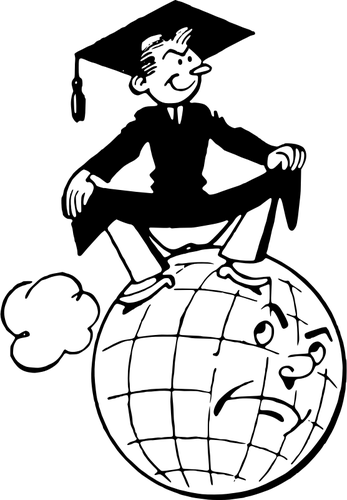
\includegraphics[width=0.22\textwidth]{img/diploma.png}
\end{wrapfigure}

Stjepan je uspješno završio preddiplomski sveučilišni studij matematike na
Prirodoslovno-matematičkom fakultetu Sveučilišta u Zagrebu. Dakako, njegovi su
roditelji jako ponosni te su mu odlučili pokloniti sve prirodne brojeve manje
ili jednake $2^{60}$. Kako ih ne bi izgubio, Stjepan je te brojeve brže-bolje
pospremio u niz $A$ tako da su brojevi poredani u neopadajućem poretku.

Njegov ljubomorni \sout{ne}prijatelj Marin odlučio mu je napakostiti te je svaki
element niza $A$ uzastopno mijenjao zbrojem njegovih znamenaka sve dok taj zbroj
nije postao jednoznamenkast. Primjerice, na 197.\ mjestu niza $A$ prvotno se
nalazio broj $197$ kojeg je Marin najprije promijenio u $1+9+7=17$, a potom u
$1+7=8$. Dakle, nakon Marinovih promjena na 197.\ mjestu niza $A$ nalazi se broj
$8$.

Stjepan je shrvan i moli Marina da vrati niz $A$ u početno stanje, ali Marin to
ne želi napraviti sve dok mu Stjepan ne odgovori na $Q$ pitanja oblika
“Kolika je suma od $l$-tog do $r$-tog elementa niza $A$ nakon mojih promjena?”.
Tek tada će Marin poštivati Stjepanovu diplomu te mu vratiti niz u početno
stanje.

Pomozite Stjepanu!

%%%%%%%%%%%%%%%%%%%%%%%%%%%%%%%%%%%%%%%%%%%%%%%%%%%%%%%%%%%%%%%%%%%%%%
% Input
\subsection*{Ulazni podaci}
U prvom je retku prirodan broj $Q$ $(1 \le Q \le 100)$ iz teksta zadatka. \\
U sljedećih su $Q$ redaka dva prirodna broja $l$ i $r$
$(1 \le l \le r \le 2^{60})$. Svaki od tih redaka predstavlja jedan Marinov
upit, a značenje brojeva $l$ i $r$ u upitu opisano je u tekstu zadatka.

%%%%%%%%%%%%%%%%%%%%%%%%%%%%%%%%%%%%%%%%%%%%%%%%%%%%%%%%%%%%%%%%%%%%%%
% Output
\subsection*{Izlazni podaci}
Potrebno je ispisati odgovore na svih $Q$ upita, a svaki je odgovor potrebno
ispisati u zasebnom retku. Naravno, na upite je potrebno odgovarati redom kako
su navedeni u ulaznim podacima.

%%%%%%%%%%%%%%%%%%%%%%%%%%%%%%%%%%%%%%%%%%%%%%%%%%%%%%%%%%%%%%%%%%%%%%
% Scoring
\subsection*{Bodovanje}
U test podacima vrijednima $10$ bodova za svaki će upit vrijediti
$1 \le l \le r \le 9$. \\
U test podacima vrijednima $30$ bodova za svaki će upit vrijediti
$r - l \le 1000$.

%%%%%%%%%%%%%%%%%%%%%%%%%%%%%%%%%%%%%%%%%%%%%%%%%%%%%%%%%%%%%%%%%%%%%%
% Examples
\subsection*{Probni primjeri}
\begin{tabularx}{\textwidth}{X'X'X}
\sampleinputs{test/trol.dummy.in.1}{test/trol.dummy.out.1} &
\sampleinputs{test/trol.dummy.in.2}{test/trol.dummy.out.2} &
\sampleinputs{test/trol.dummy.in.3}{test/trol.dummy.out.3}
\end{tabularx}

\textbf{Pojašnjenje drugog probnog primjera:}

\textbf{1. upit} \textrightarrow{}
$A_9 = 9$, $A_{10} = 1 + 0 = 1$, $A_{11} = 1 + 1 = 2$,
$A_{12} = 1 + 2 = 3$, $A_{13} = 1 + 3 = 4$.\\
\phantom{\textbf{1. upit} \textrightarrow{}}
$A_9 + A_{10} + A_{11} + A_{12} + A_{13} = 9 + 1 + 2 + 3 + 4 = 19$.

\textbf{2. upit} \textrightarrow{}
$A_{44} = 4 + 4 = 8$, $A_{45} = 4 + 5 = 9$. $A_{44} + A_{45} = 8 + 9 = 17$.

%%%%%%%%%%%%%%%%%%%%%%%%%%%%%%%%%%%%%%%%%%%%%%%%%%%%%%%%%%%%%%%%%%%%%%
% We're done
\end{statement}

%%% Local Variables:
%%% mode: latex
%%% mode: flyspell
%%% ispell-local-dictionary: "croatian"
%%% TeX-master: "../hio.tex"
%%% End:
